\title{Solana: Une nouvelle architecture pour une blockchain haute performance v0.8.14 }

\author{
        Anatoly Yakovenko \\
        anatoly@solana.io\\
}
\date{}

\documentclass[12pt]{article}

% \usepackage{draftwatermark}
% \SetWatermarkText{Confidential}
% \SetWatermarkScale{5}
% \SetWatermarkColor[gray]{0.95}

\usepackage{graphicx}
\usepackage{bytefield}
\usepackage{makecell}
\usepackage[utf8]{inputenc}
\usepackage[T1]{fontenc}

\usepackage[]{hyperref}
\hypersetup{
    pdftitle={Solana: A new architecture for a high performance blockchain},
    pdfauthor={anatoly@solana.io},
    pdfsubject={blockchain},
    pdfkeywords={blockchain, bitcoin, cryptocurrency},
    bookmarksnumbered=true,
    bookmarksopen=true,
    bookmarksopenlevel=1,
    colorlinks=true,
    pdfstartview=Fit,
    pdfpagemode=UseOutlines,    % this is the option you were lookin for
    pdfpagelayout=TwoPageRight
}

\begin{document}
\maketitle

\textbf{\footnotesize Avertissement légal}\scriptsize
~~Rien de ce qui figure dans ce White Paper n'est une offre de vente, ou la sollicitation d'une offre d'achat ou de token. Solana publie ce White Paper uniquement pour collecter des informations et des commentaires du public. Si et lorsque Solana mettra en vente des tokens (ou un Simple Accord pour de futurs tokens, elle le fera par le biais de documents d'offre définitifs, y compris un document d'information comprenant également les facteurs de risque. Ces documents définitifs devraient également inclure une version mise à jour de ce White Paper, qui pourrait différer sensiblement de la version actuelle. Si et quand Solana fait une telle offre aux États-Unis, l'offre sera probablement disponible uniquement pour les investisseurs accrédités.

Rien dans ce White Paper ne doit être considéré ou interprété comme une garantie ou une promesse de développement de l'activité ou des tokens de Solana ou de l'utilité ou de la valeur des tokens. Ce White Paper expose les plans actuels, qui pourraient changer à sa discrétion, et dont le succès dépendra de nombreux facteurs indépendants de la volonté de Solana, entre autres les facteurs dépendants du marché et des facteurs des industries de données et de crypto-monnaie. Toute déclaration concernant des événements futurs est basée uniquement sur l'analyse de Solana des problèmes décrits dans ce White Paper. Cette analyse pourrait s’avérer incorrecte.

\begin{abstract}
Cet article propose une nouvelle architecture de blockchain basée sur la Proof of History (PoH) - une preuve pour vérifier l'ordre et le temps écoulé entre les événements. PoH est utilisé pour encoder le " temps incertain " dans un registre – constituant seulement un complément de données. Lorsqu'il est utilisé avec un algorithme de consensus comme le Proof of Work (PoW) ou Proof of Stack (PoS), PoH peut réduire la surcharge de messages dans une machine " à tolérance d’erreurs " (répliquée Byzantine), permettant un temps de traitement de moins d’une seconde. Cet article propose également deux algorithmes qui exploitent les propriétés de conservation du temps du registre PoH - un algorithme de PoS qui peut récupérer à partir de partitions de toute taille et une Proof of Replication (PoRep). La combinaison de PoRep et PoH assure une protection contre la falsification du grand livre en ce qui concerne le temps (commande) et le stockage. Le protocole est analysé sur un réseau $1$~gbps, et cet article montre que le débit peut atteindre $710$k transactions par seconde avec le matériel actuel.
\end{abstract}


\section{Introduction}\normalsize
Blockchain est l’implémentation d'une machine tolérante aux pannes. Les blockchains disponibles publiquement ne dépendent pas du temps, ou font une faible hypothèse sur les capacités du participant à garder le temps~\cite{tendermint,hashgraph}. Chaque nœud du réseau s'appuie généralement sur sa propre horloge locale sans connaître les horloges des autres participants du réseau. L'absence d'une source fiable de temps signifie que lorsqu'un horodatage de message est utilisé pour accepter ou rejeter un message, il n'y a aucune garantie que tous les autres participants du réseau feront exactement le même choix. Le PoH présenté ici est conçu pour créer un registre avec un passage vérifiable du temps, c'est-à-dire la durée entre les événements et l'ordre des messages. Il est prévu que chaque nœud du réseau pourra compter sur le passage du temps enregistré dans le registre sans confiance.

\section{Contour}
Le reste de cet article est organisé comme suit. La conception globale du système est décrite dans la section~\ref{design}. La description détaillée de la Proof of History est décrite dans la section~\ref{proof_of_history}. La description détaillée de l'algorithme de consensus proposé Proof of Stake est décrite dans la section~\ref{proof_of_stake}. Une description détaillée de la Proof of Replication proposée se trouve dans la section~\ref{porep}. L'architecture du système et les limites de performance sont analysées dans la section~\ref{system_architecture}. Un moteur GPU de smart-contract intuitif haute perfomance est décrit dans la Section~\ref{sec:smartcontracts}

\section{Conception du réseau}\label{design}

\begin{figure}[h]
  \begin{center}
    \centering
    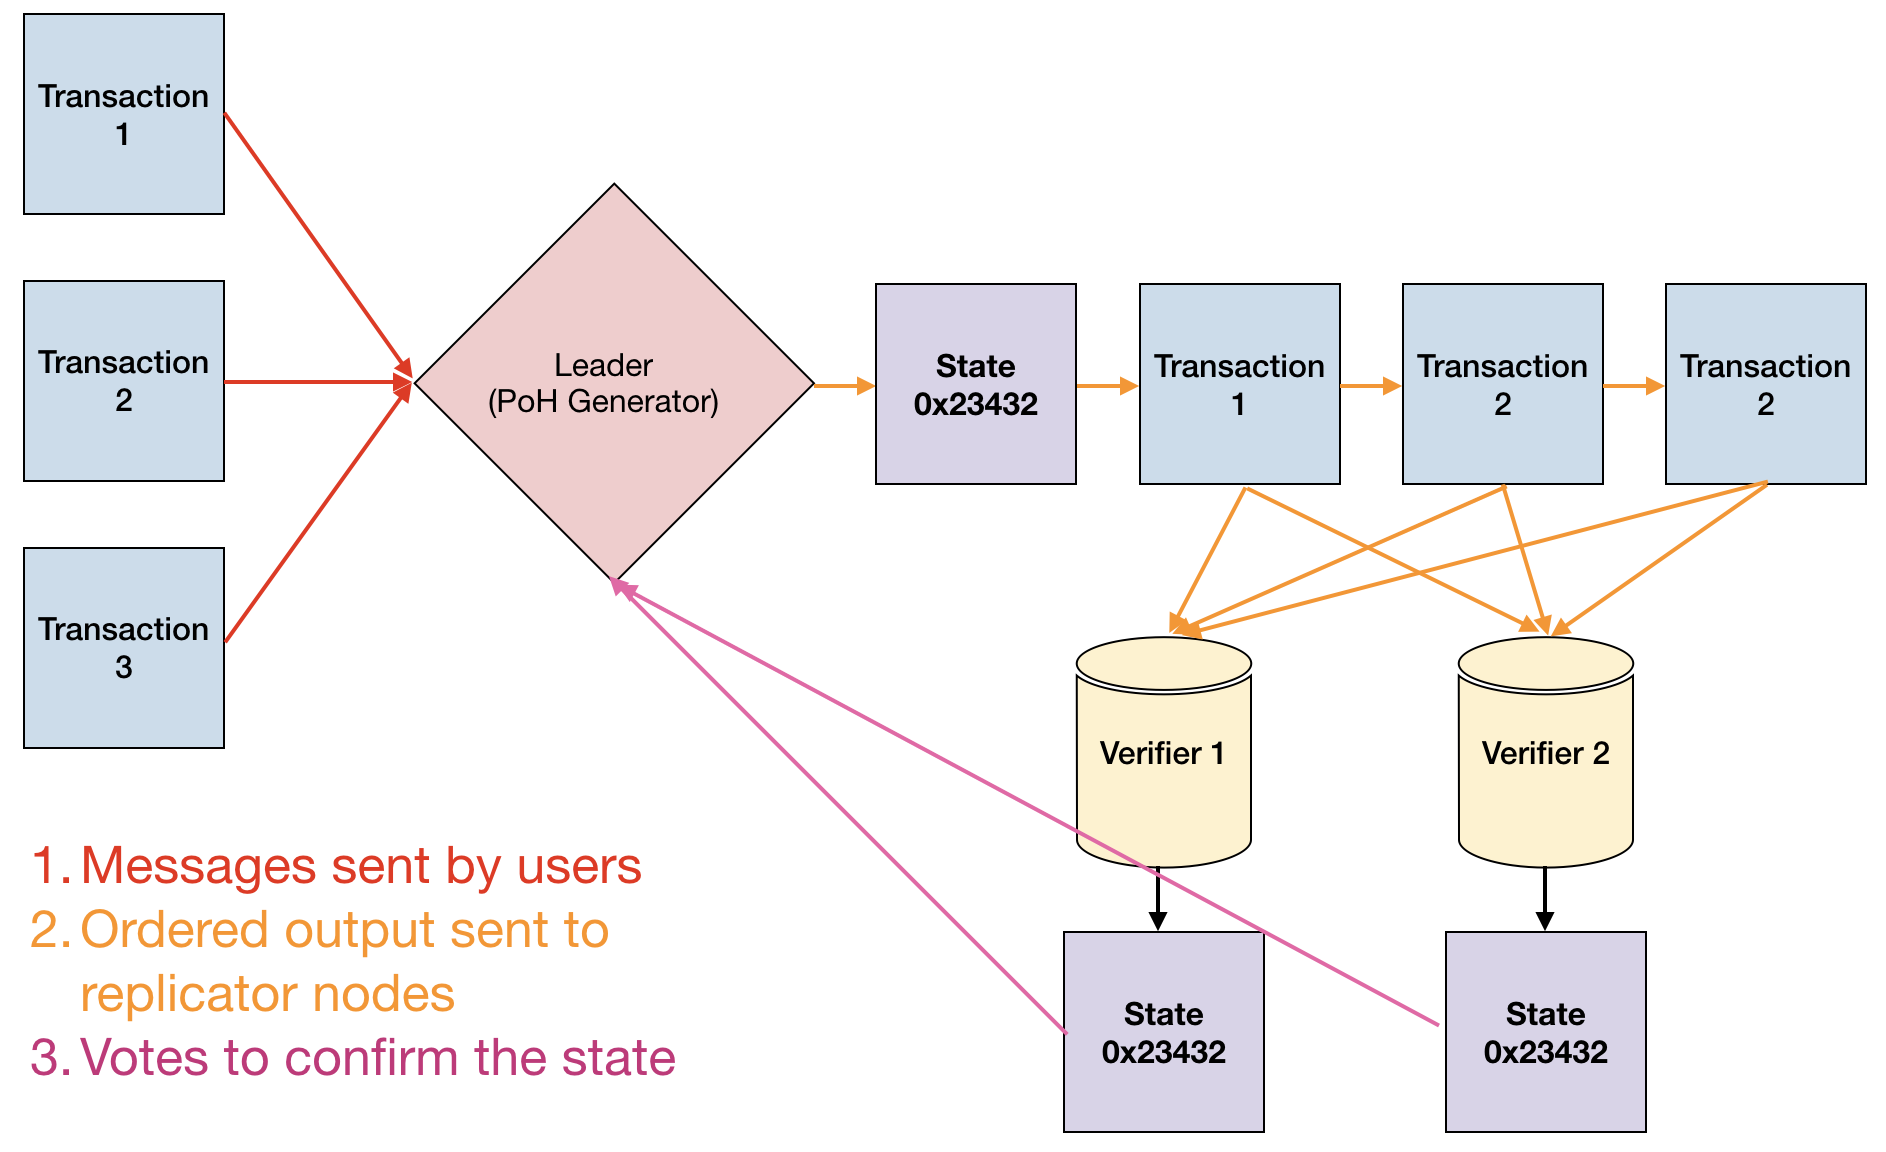
\includegraphics[width=\textwidth]{figures/network_design_001.png}
    \caption[Fig 1]{Transaction flow throughout the network.\label{fig:design}}
  \end{center}
  \end{figure}

Comme représenté sur l’image~\ref{fig:design}, un nœud de système est désigné à tout moment comme " Leader " pour générer une séquence de " Proof of History ", garantissant la cohérence de lecture globale du réseau et un passage de temps vérifiable. Le leader séquence les messages d'utilisateur et les classe de manière à ce qu'ils puissent être traités efficacement par d'autres nœuds du système, maximisant ainsi le débit. Il exécute les transactions sur l'état actuel qui est stocké dans la " RAM " et publie les transactions et une signature de l'état final sur les nœuds de réplication appelés Vérificateurs. Les Vérificateurs exécutent les mêmes transactions sur leurs copies de l'état, et publient leurs signatures enregistrées en tant que confirmations. Les confirmations publiées servent de votes pour l'algorithme de consensus.

Dans un état non classé (partitionné), à un moment donné, il y a un Leader dans le réseau. Chaque noeud vérificateur a les mêmes capacités matérielles qu'un Leader et peut être élu en tant que Leader, ceci se fait via des élections basées sur le PoS. Les élections pour l'algorithme de PoS proposé sont traitées en détail dans la Section~\ref{subsec:elections}.

En termes de théorème de CAP, la cohérence est presque toujours choisie en fonction de la disponibilité dans un événement d'une partition. Dans le cas d'une grande partition, cet article prévoit un mécanisme pour récupérer le contrôle du réseau à partir d'une partition de n'importe quelle taille. Ceci est expliqué en détail dans la Section~\ref{disponibility}.

\section{Proof of History}\label{proof_of_history}

La " Proof of History " est une séquence de calcul qui peut fournir un moyen de vérifier cryptographiquement le passage du temps entre deux événements. Il utilise une fonction cryptographiquement sécurisée écrite afin que la sortie ne puisse pas être définie par l'entrée, et doit être complètement exécutée pour générer la sortie. La fonction est exécutée dans une séquence sur un seul noyau, sa sortie précédente étant l'entrée actuelle, l'enregistrement périodique de la sortie actuelle et le nombre de fois qu'elle a été appelée. La sortie peut ensuite être recalculée et vérifiée par des ordinateurs externes en parallèle en vérifiant chaque segment de séquence sur un noyau séparé.

Les données peuvent être horodatées dans cette séquence en ajoutant les données (ou un hash de certaines données) dans l'état de la fonction. L'enregistrement de l'état, de l'index et des données tels qu'ils ont été ajoutés dans les séquences fournit un horodatage qui peut garantir que les données ont été créées avant que le hachage suivant ne soit généré dans la séquence. Cette conception prend également en charge la mise à l'échelle horizontale car plusieurs générateurs peuvent se synchroniser entre eux en mélangeant leur état dans les séquences des autres. La mise à l'échelle horizontale est discutée en profondeur dans la Section~\ref{poh:mise_echelle}\\

\subsection{Description}
Le système est conçu pour fonctionner comme suit.  Avec une fonction de hash cryptographique, dont la sortie ne peut être prédite sans exécuter la fonction (e.g. \texttt{sha256}, \texttt{ripemd}, etc.),  exécuter la fonction à partir d'une valeur de départ aléatoire et prendre sa sortie comme entrée dans la même fonction à nouveau. Noter le nombre de fois que la fonction a été appelée et la sortie à chaque appel. La valeur aléatoire de départ choisie peut être n'importe quelle chaîne, comme le titre du jour du New York Times.
\\\\
\noindent Par exemple: \noindent
\begin{center}
  \begin{tabular}{  l  l  r }
%    \hline
    \multicolumn{3}{c}{PoH Sequence} \\
    \hline
    Index  & Operation & Output Hash \\ \hline
    $1$ & sha256(\char`\"any random starting value\char`\") & \texttt{hash1}\\ %\hline
    $2$ &  sha256(\texttt{hash1}) & \texttt{hash2}\\ %\hline
    $3$ & sha256(\texttt{hash2}) & \texttt{hash3}\\ %\hline
    \end{tabular}
\end{center}

\noindent Où \texttt{hashN} représente le resultat de hash actuel.\\

Il est seulement nécessaire de publier un sous-ensemble des hashes et des index à un intervalle.\\

\noindent Par exemple:\\\\\noindent
\begin{center}
  \begin{tabular}{ l  l  r }
    \multicolumn{3}{c}{PoH Sequence} \\
    \hline
    Index & Operation & Output Hash \\ \hline
    $1$ & sha256(\char`\"any random starting value\char`\") & \texttt{hash1}\\
    $200$ &  sha256(\texttt{hash199}) & \texttt{hash200}\\
    $300$ & sha256(\texttt{hash299}) & \texttt{hash300} \\
    \end{tabular}
\end{center}

Tant que la fonction de hash choisi est résistante aux collisions, cet ensemble de hashes ne pourra être calculé en séquence que par un seul thread. Cela vient du fait qu’il n’est pas possible de prédire quelle sera la valeur du hash à l'index $300$ sans lancer l’algorithme depuis le début $300$ fois. On peut donc déduire de la structure de données que du temps réel s’est écoulé entre l’index $0$ et l'index $300$.

Dans l’exemple de la Figure~\ref{fig:poh_seq}, hash \texttt{62f51643c1} a été produit au comptage $510144806912$ et le hash \texttt{c43d862d88} a été produit au
comptage $510146904064$. Suivant les propriétés précédemment énoncées de l’algorithme PoH, nous pouvons en déduire que le temps réel s’est écoulé entre le compte $510144806912$
et le compte $510146904064$.

\begin{figure}[h]
  \begin{center}
    \centering
    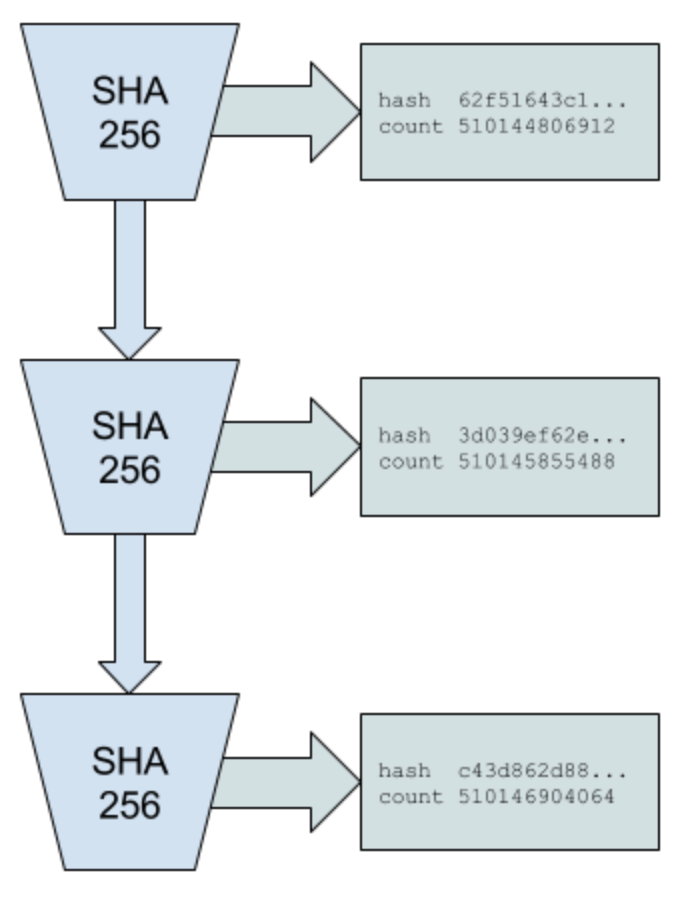
\includegraphics[width=0.5\textwidth]{figures/poh_sequence_001.png}
    \caption[Figure 2]{Séquence de Proof of History\label{fig:poh_seq}}
  \end{center}
  \end{figure}

\subsection{Horodatage des événements}

Cette séquence de hashes peut aussi être utilisée pour enregistrer le fait que certaines données aient été créées avant qu’un certain index hash soit généré. En utilisant une " fonction combinée " pour combiner les données avec le hash actuel à l’index actuel. Les données peuvent simplement être un unique hash d’événements arbitraires. La fonction combinée peut être un simple ajout de données ou n’importe quelle opération qui est résistante aux collisions. Le hash généré par la suite représente un horodatage des données parce que ce hash n’aurait pu être généré seulement après que ces données ne soient insérées.\\

\noindent Par exemple:\\\\\noindent
\begin{center}
  \begin{tabular}{ l l r }
    \multicolumn{3}{c}{PoH Sequence} \\
    \hline
    Index  & Operation  & Output Hash\\ \hline
    $1$ & sha256(\char`\"any random starting value\char`\") & \texttt{hash1}\\
    $200$ & sha256(\texttt{hash199}) & \texttt{hash200}\\
    $300$ & sha256(\texttt{hash299}) & \texttt{hash300}\\
    \end{tabular}
\end{center}


\noindent Si un événement externe survient, comme une photo qui est prise ou la création arbitraire d’une donnée digitale:\\\\\noindent
\begin{center}
  \begin{tabular}{ l l r}
    \multicolumn{3}{c}{PoH Sequence With Data} \\
    \hline
    Index  & Operation & Output Hash\\ \hline
    $1$ & sha256(\char`\"any random starting value\char`\") & \texttt{hash1} \\
    $200$ & sha256(\texttt{hash199}) & \texttt{hash200} \\
    $300$  & sha256(\texttt{hash299}) & \texttt{hash300}\\
    $336$ & sha256(append(\texttt{hash335}, photograph\_sha256)) & \texttt{hash336}\\
    \end{tabular}
\end{center}


\texttt{Hash336} est calculé à partir de la donnée binaire ajoutée du
\texttt{hash335} et du \texttt{sha256} de la photo. L’index
et le \texttt{sha256} de la photo sont enregistrées en tant que partie de la
séquence générée. Dès lors, quiconque vérifiant cette séquence peut ensuite recréer
ce changement à cette séquence. La vérification peut toujours être effectuée en
parallèle et est expliquée dans la Section~\ref{poh:verify}

Etant donné que le procédé initial est toujours séquentiel, nous pouvons en déduire que les éléments introduits dans la séquence ont dû se dérouler avant que la prochaine valeur de hash soit calculée.

\begin{center}
  \begin{table}
  \begin{tabular}{l l r}
    \multicolumn{3}{c}{POH Sequence} \\ \hline
    Index & Operation & Output Hash \\ \hline
    $1$ & sha256(\char`\"any random starting value\char`\") & \texttt{hash1} \\
    $200$ & sha256(hash199) & \texttt{hash200} \\
    $300$ & sha256(hash299) & \texttt{hash300} \\
    $336$ & sha256(append(hash335, photograph1\_sha256)) & \texttt{hash336}\\
    $400$ & sha256(hash399) & \texttt{hash400} \\
    $500$ & sha256(hash499) & \texttt{hash500}\\
    $600$ & sha256(append(hash599, photograph2\_sha256)) & \texttt{hash600}\\
    $700$ & sha256(hash699) & \texttt{hash700}\\
    \end{tabular}
    \caption[Table 1]{Séquence PoH avec 2 évènements\label{table:multievent}}
    \end{table}
\end{center}

Dans la séquence reprise dans la Table~\ref{table:multievent}, \texttt{photograph2} a été créée avant le \texttt{hash600}, et la
\texttt{photograph1} a été créée avant le \texttt{hash336}. Insérer la donnée dans la séquence de hashes produit un changement pour toutes les valeurs dans la séquence. Tant que la fonction de hash utilisée est résistante aux collisions, et que la donnée est ajoutée, il devrait être mathématiquement impossible de pré-calculer une séquence future sur base de connaissance passée relative à quelle donnée sera intégrée dans la séquence.\\

La donnée qui est mixée à la séquence peut être la donnée brute ou seulement un hash de la donnée accompagnée de métadonnées.\\

\begin{figure}[h]
  \begin{center}
    \centering
    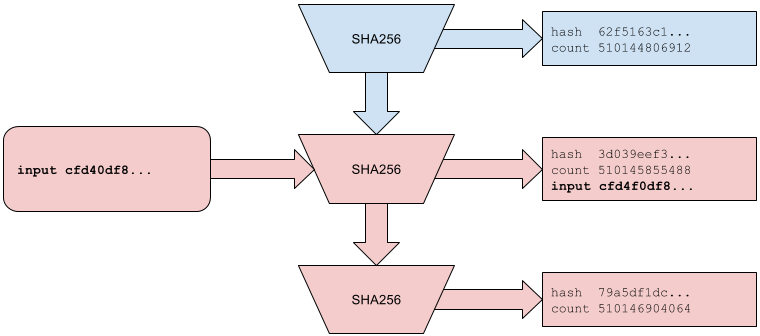
\includegraphics[width=0.9\textwidth]{figures/fig_3.png}
    \caption[Fig 3]{Insertion de données à la Proof of History\label{fig:poh_insert}}
  \end{center}
  \end{figure}

  Dans l’exemple en  Figure~\ref{fig:poh_insert}, l'input \texttt{cfd40df8\ldots} a été inséré dans la séquence de Proof of History. Le comptage auquel l’input a été inséré est $510145855488$ et l’état auquel il a été inséré est \texttt{3d039eef3}. Tous les prochains hashes générés sont impactés par ce changement de séquence. Ce changement est indiqué par le changement de couleur dans la figure.\\

Chaque node observant la séquence peut déterminer l’ordre dans lequel chaque événement a été inséré et peut déterminer le temps réel entre chaque insertion.

\subsection{Vérification}\label{poh:verify}
La séquence peut être vérifiée par un ordinateur multi-coeur en moins de temps qu’il ne faut pour la générer.\\

\noindent Par exemple: \\\noindent

\begin{center}

\begin{tabular}{l l r}
    \multicolumn{3}{c}{Coeur 1} \\ \hline
    Index & Data & Output Hash \\ \hline
    $200$ & sha256(\texttt{hash199}) & \texttt{hash200} \\
    $300$ & sha256(\texttt{hash299}) & \texttt{hash300}\\
    \end{tabular}\\

  \begin{tabular}{l l r}
    \multicolumn{3}{c}{Coeur 2} \\
    \hline
    Index & Data & Output Hash \\ \hline
    $300$ & sha256(\texttt{hash299}) & \texttt{hash300} \\
    $400$ & sha256(\texttt{hash399}) & \texttt{hash400}\\
    \end{tabular}

\end{center}


Pour un certain nombre de coeurs donnés, comme un GPU moderne avec $4000$ coeurs, le vérificateur peut séparer la séquence de hashes et leurs indexes en $4000$ tranches, et en parallèle, assurer que chaque tranche est correcte du premier au dernier hash de la tranche. Si le temps prévu pour produire la séquence est:\\


\[
\frac{\textrm{Nombre total de Hashes}}{\textrm{Hashes par seconde pour 1 coeur}}
\]

\noindent Le temps estimé pour vérifier qu’une séquence soit effectivement correcte est:\\

\[
\frac{\textrm{Nombre total de Hashes}}{\textrm{(Hashes par seconde et par coeur * Nombre de coeur disponible à la vérification)}}
\]

\begin{figure}
  \begin{center}
    \centering
    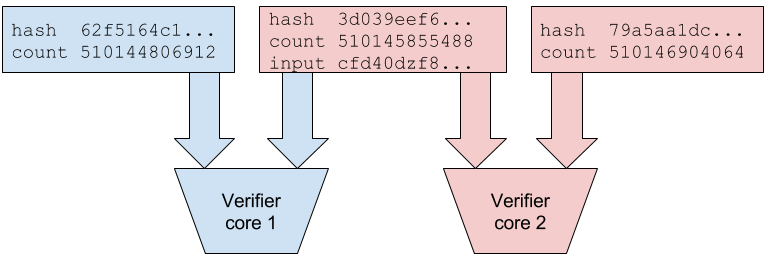
\includegraphics[width=0.9\textwidth]{figures/fig_4.png}
    \caption[Figure 4]{Vérification utilisant plusieurs coeurs\label{fig:poh_verification}}
  \end{center}
  \end{figure}

En exemple, la figure ~\ref{fig:poh_verification}, chaque cœur est capable de vérifier individuellement chaque partie de la séquence en parallèle. Puisque toutes les données en entrée sont enregistrées au niveau de la sortie, avec également le compteur et l'état auquel ils sont attachés, les vérificateurs peuvent répliquer chaque partie en parallèle. Les hashes (en rouge ici plus haut) indiquent que la séquence était modifiée par une insertion de données.

\subsection{Mise à l'échelle Horizontale}\label{poh:mise_echelle}
Il est possible de synchroniser plusieurs " Proof of History " en mélangeant
l'état de la séquence de chaque générateur avec un second générateur, et ainsi atteindre
la mise à l'échelle horizontale du générateur " Proof of History ". Cette mise à l'échelle est faite
sans " sharding ". Le résultat des deux générateurs est nécessaire pour reconstruire
l'ordre complet des événements dans le système.

\begin{center}
  \begin{tabular}{|l c r|}

  \hline
    \multicolumn{3}{|c|}{PoH Générateur  A} \\
  %  \hline
    Index & Hash & Data \\ \hline
    $1$ & \texttt{hash1a} & \\
    $2$ & \texttt{hash2a} & \texttt{hash1b} \\
    $3$ & \texttt{hash3a} & \\
    $4$ & \texttt{hash4a} & \\
    \hline
    \end{tabular}
  \begin{tabular}{| l  c  r |}
  \hline
    \multicolumn{3}{|c|}{PoH Générateur B} \\
%    \hline
    Index & Hash & Data \\ \hline
    $1$ & \texttt{hash1b} & \\
    $2$ & \texttt{hash2b} & \texttt{hash1a} \\
    $3$ & \texttt{hash3b} & \\
    $4$ & \texttt{hash4b} & \\
    \hline
    \end{tabular}
\end{center}

Imaginons les générateurs A et B, A reçoit un paquet de données de B (hash1b), qui contient le dernier état du générateur B, et le dernier état du générateur B observé sur le générateur A. L'état suivant du générateur A dépend alors de l'état de Générateur B, donc nous pouvons déduire que hash1b est arrivé avant hash3a. Cette propriété peut être transitive, donc si trois générateurs sont synchronisés via un seul générateur commun \(A \leftrightarrow B \leftrightarrow C \), nous pouvons tracer la dépendance entre A et C même s'ils ne sont pas synchronisés directement.

En synchronisant périodiquement les générateurs, chaque générateur peut alors gérer une partie du trafic externe, ainsi le système global peut gérer un plus grand nombre d'événements à traquer et cela au prix d'une précision en temps réel (dépendent de la latence du réseau entre les générateurs). Un ordre global peut encore être obtenu en choisissant une fonction déterministe qui pourra invoquer tous les événements qui se trouvent dans la fenêtre de synchronisation, comme par exemple la valeur du hash lui-même.


\begin{figure}
  \begin{center}
    \centering
    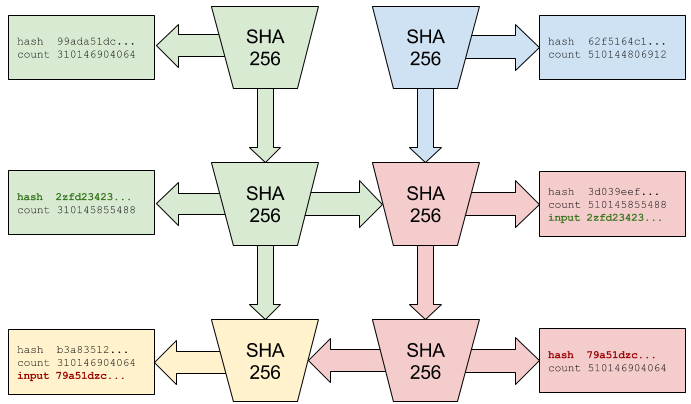
\includegraphics[width=0.9\textwidth]{figures/fig_5.png}
    \caption[Fig 5]{Deux générateurs se synchronisant\label{fig:poh_mise_echelle}}
  \end{center}
  \end{figure}

Sur la figure~\ref{fig:poh_mise_echelle}, les deux générateurs utilisent la sortie de l'autre et enregistrent l'opération. Le changement de couleur indique que les données de l’autre partie ont modifié la séquence. Les hashes générés qui sont mélangés dans chaque flux sont surlignés en gras.

La synchronisation est transitive. \(A \leftrightarrow B \leftrightarrow C\)  Il existe un ordre d'événements prouvable entre A et C à travers B.

%% Il est à noter que les $710$k tx/s théoriques sur un réseau $1$ ~ gb basé sur la conception de PoH ne tiennent pas compte de la capacité supplémentaire offerte par la mise à l'échelle horizontale.
De cette manière, la mise à l'échelle se fait au détriment de la disponibilité. Des connections $10 \times 1$~gbps avec une disponibilité de 0.999 auraient une disponibilité de \(0.999^{10} = 0.99 \).

\subsection{Consistance}
Les utilisateurs doivent pouvoir renforcer la consistance de la séquence générée et la rendre résistante aux attaques en insérant la dernière sortie observée de la séquence qu'ils considèrent comme valide, dans leur entrée.\\

\begin{center}
  \begin{tabular}{ | l c r |}
    \hline
    \multicolumn{3}{|c|}{PoH Sequence A} \\
    Index & Data & Output Hash  \\ \hline
    $10$ & & \texttt{hash10a} \\
    $20$ & Event1 & \texttt{hash20a} \\
    $30$ & Event2 & \texttt{hash30a} \\
    $40$ & Event3 & \texttt{hash40a} \\
    \hline
    \end{tabular}
  \begin{tabular}{ | l c r |}
    \hline
    \multicolumn{3}{|c|}{PoH Hidden Sequence B} \\
    Index & Data & Output Hash \\ \hline
    $10$ & & \texttt{hash10b}\\
    $20$ & Event3 & \texttt{hash20b}  \\
    $30$ & Event2 & \texttt{hash30b} \\
    $40$ & Event1 & \texttt{hash40b} \\
    \hline
    \end{tabular}
\end{center}

Un générateur PoH malveillant peut produire une deuxième séquence cachée avec les événements dans l'ordre inverse et ce, s’il a accès à tous les événements à la fois ou s’il est capable de générer une séquence cachée plus rapide.\\

Pour éviter cette attaque, chaque événement généré par le client doit contenir le dernier hash observé de ce qu'il considère être une séquence valide. Ainsi, lorsqu'un client crée la donnée "Event1", il doit ajouter le dernier hash observé.\\

\begin{center}
  \begin{tabular}{  l  c l}

    \multicolumn{3}{c}{PoH Séquence A} \\
    \hline
    Index  & Data & Output Hash  \\ \hline
    $10$ & & \texttt{hash10a} \\
    $20$ & Event1 = append(event1 data, \texttt{hash10a}) & \texttt{hash20a}  \\
    $30$ & Event2 = append(event2 data, \texttt{hash20a}) & \texttt{hash30a} \\
    $40$ &  Event3 = append(event3 data, \texttt{hash30a}) & \texttt{hash40a} \\
    \end{tabular}
\end{center}

Lorsque la séquence est publiée, Event3 fait référence à hash30a, et si ce n'est pas dans la séquence précédente à cet événement, les consommateurs de la séquence savent qu'il s'agit d'une séquence invalide. L'attaque de " réarrangement partiel " serait alors limitée au nombre de hashes produits durant le laps de temps où le client a observé un événement et ce, depuis son entré. Les clients devraient alors être en mesure d'écrire des softwares qui ne supposent pas que l'ordre soit correct pour la courte période de hashes entre le dernier hash observé et inséré.

Pour empêcher un générateur PoH malveillant de réécrire les hashes des évènements clients, les clients peuvent soumettre une signature des données d'événement ainsi que le dernier hash observé au lieu de simplement soumettre les données.\\
\begin{center}
  \begin{tabular}{  l  l  r }
    \multicolumn{3}{c}{PoH Séquence A} \\
    \hline
    Index & Data & Output Hash \\ \hline
    $10$ & & hash10a  \\
    $20$ & \makecell{Event1 = sign(append(event1 data, hash10a), \\Client Private Key)} & hash20a\\
    $30$ & \makecell{Event2 = sign(append(event2 data, hash20a), \\Client Private Key)} & hash30a \\
    $40$ & \makecell{Event3 = sign(append(event3 data, hash30a), \\Client Private Key)} & hash40a \\

    \end{tabular}
\end{center}

La vérification de ces données nécessite une vérification de signature ainsi qu’une vérification du hash dans la séquence de hachage précédente.\\
\noindent Vérification:\\

\noindent\texttt{(Signature, PublicKey, hash30a, event3 data) = Event3} \\
\texttt{Verify(Signature, PublicKey, Event3)}\\
\texttt{Lookup(hash30a, PoHSequence)}\\

\begin{figure}
  \begin{center}
    \centering
    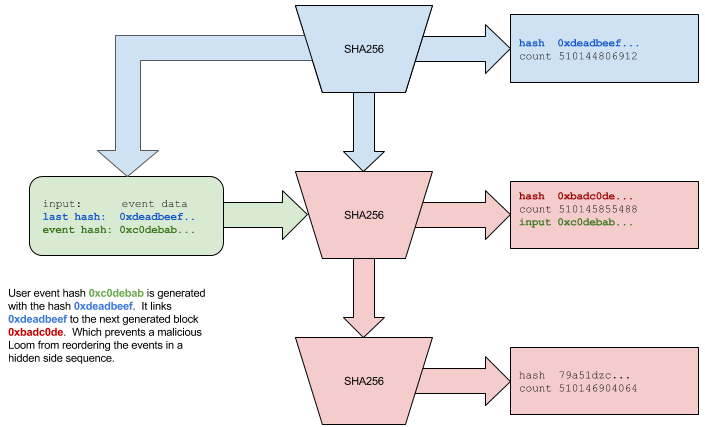
\includegraphics[width=0.9\textwidth]{figures/fig_6.png}
    \caption[Fig 6]{Hash précédent en tant que donnée d'entrée.\label{fig:poh_consistance}}
  \end{center}
  \end{figure}

Dans la figure~\ref{fig:poh_consistance}, l’entrée fournie par l’utilisateur dépend du hash \texttt{0xdeadbeef\ldots} existant dans la séquence générée avant son insertion. La flèche bleue en haut à gauche indique que le client fait référence à un hash précédemment produit. Le message du client n'est valide que dans une séquence contenant le hash \texttt{0xdeadbeef\ldots}. La couleur rouge de la séquence indique que la séquence a été modifiée par les données du client.

\subsection{Overhead}
4000 hashes par seconde généreraient 160 kilo-octets de données supplémentaires, et nécessiteraient l'accès à un GPU avec 4000 noeuds et un temps de vérification d'environ 0,25-0,75 millisecondes..

\subsection{Attaques}
\subsubsection{Annulation}
 La génération d'un ordre inverse nécessiterait qu'un attaquant lance la séquence malveillante après le second événement. Ce délai devrait permettre à tous les nœuds  " d’égal à égal "  non malveillants de communiquer sur l'ordre original

\subsubsection{Vitesse}
Avoir plusieurs générateurs peut rendre le déploiement plus résistant aux attaques. Un générateur peut avoir une "bande passante élevée et recevoir de nombreux événements à mélanger dans sa séquence, un autre générateur pouvant être une bande passante à haut débit qui se mélange périodiquement avec le générateur à bande passante élevée.

La séquence à haute vitesse créerait une séquence secondaire de données qu'un attaquant devrait inverser.

\subsubsection{Attaques à longue portée}

Les attaques à longue portée impliquent l'acquisition d’anciennes clés privées de clients abandonnées et la génération d'un registre falsifié ~\cite{casper}. La preuve historique assure une certaine protection contre les attaques à longue portée. Un utilisateur malveillant qui accède aux anciennes clés privées doit recréer un historique qui demandera autant d'effort de création qu'en a nécessité l'original. Cela nécessiterait l'accès à un processeur plus rapide que celui actuellement utilisé par le réseau, sinon l'attaquant ne rattraperait jamais la longueur de l'historique.

De plus, une seule source de temps permet la construction d'une preuve de réplication plus simple (plus de détails dans la section ~\ref{porep}), puisque le réseau est conçu de sorte que tous les participants du réseau s'appuient sur un seul enregistrement historique des événements.

PoRep et PoH ensemble devraient fournir une défense spatiale et temporelle contre la constitution d'un faux registre.


\section{Proof of Stake Consensus}\label{proof_of_stake}
\subsection{Description}
Cette instance spécifique de " Proof of Stake " est conçue pour la confirmation rapide de la séquence actuelle produite par le générateur " Proof of History ", pour le vote et la sélection du générateur de preuve historique suivant, et pour punir les validateurs malveillants. Cet algorithme dépend des messages qui arrivent finalement à tous les nœuds participants dans un certain délai.
\subsection{Terminologie}
\begin{description}

\item[obligations]
Les obligations sont équivalentes à une dépense en capital dans un système de " Preuve de travail ". Un mineur achète du matériel et de l'électricité et le confie à une seule succursale dans une blockchain " Proof of Work ". Une obligation est une pièce servant de garantie pendant la validation des transactions.

\item[slashing]

La solution proposée au problème du " rien en jeu " dans les systèmes de preuve de participation ~\cite{slasher}. Lorsqu'une preuve de vote pour une autre succursale est publiée, cette succursale peut annuler la caution du validateur. Ceci est une incitation économique conçue pour décourager les validateurs de confirmer plusieurs branches.
\item[super majorité]
Une super majorité est \(\frac{2}{3}\) des validateurs pondérés par leurs liens. Un vote majoritaire indique que le réseau a atteint un consensus, et qu'au moins \(\frac{1}{3}\) du réseau aurait dû voter de façon malveillante pour que cette branche soit invalide. Cela mettrait le coût économique d'une attaque à \(\frac{1}{3}\) de la capitalisation boursière de la pièce.

\end{description}

\subsection{Obligations}
Une transaction de liaison implique une quantité de pièces de monnaie spécifiée par un utilisateur qui la transfert vers un compte lié à son identité. Les pièces dans le compte de cautionnement ne peuvent pas être dépensées et doivent rester dans le compte jusqu'à ce que l'utilisateur les supprime. L'utilisateur ne peut supprimer que les pièces périmées qui ont expiré. Les obligations ne sont valables qu’après que la ‘super majorité’ (grande majorité) des parties prenantes ait confirmé la séquence.

\subsection{Vote}
Il est prévu que le générateur " Proof of History " puisse publier une signature de l'état à une période prédéfinie. Chaque identité liée doit confirmer cette signature en publiant sa propre signature signée de l'état. Le vote est un simple vote oui, (sans un non).  Si la majorité des identités liées a voté dans un délai d’attente déterminé, cette branche sera acceptée comme valable.

\subsection{Suppression de vote}

Un nombre N de voix manquantes indique que les pièces sont périmées et ne sont plus éligibles pour le vote. L'utilisateur peut émettre une transaction non liée pour les supprimer.

N est une valeur dynamique basée sur le rapport entre les votes périmés et actifs. N augmente à mesure que le nombre de votes périmés augmente. Dans le cas d'une partition réseau importante, cela permet à la branche la plus importante de récupérer plus rapidement que la branche plus petite.

\subsection{Elections}\label{subsec:elections}
L'élection d'un nouveau générateur de PoH se produit lorsque la défaillance du générateur PoH est détectée. Le validateur ayant la plus grande puissance de vote, ou l'adresse de clé publique la plus élevée en cas d'égalité, est choisi comme nouveau générateur de PoH.

Une super majorité de confirmations est requise sur la nouvelle séquence. Si le nouveau leader échoue avant qu'une confirmation de super-majorité ne soit disponible, le validateur le plus élevé suivant est sélectionné, et un nouvel ensemble de confirmations est requis.

Pour changer de vote, un validateur doit voter à un compteur de séquence PoH plus élevé, et le nouveau vote doit contenir les votes qu'il veut changer. Sinon, le deuxième vote pourra être annulé " slashable ". Le changement de vote devrait être conçu de manière à ce qu'il ne puisse avoir lieu qu'à un niveau non majoritaire.

Une fois qu'un générateur de PoH est établi, un générateur suppléant peut être choisi pour prendre en charge les tâches de traitement transactionnel. Si un deuxième existe, il sera considéré comme le prochain leader lors d'une défaillance primaire.

La plate-forme est conçue pour que le suppléant devienne primaire et que les générateurs de rang inférieur soient promus si une anomalie est détectée ou selon un calendrier prédéfini.
\subsection{Déclencheurs d'élection}
\subsubsection{Forked Proof of History generator}

Les générateurs de PoH sont conçus avec une identité qui signe la séquence générée. Une " fourchette " ne peut apparaître que si l'identité du générateur PoH a été compromise. Une " fourchette " est détectée car deux enregistrements historiques différents ont été publiés sur la même identité PoH.

\subsubsection{Exceptions au Runtime}
Un bug, une défaillance ou une erreur intentionelle dans le générateur de PoH pourrait faire en sorte que ce dernier génère un état invalide et publie une signature d'état ne correspondant pas au résultat du validateur local.  Les validateurs vont publier la signature correcte \textit{via gossip} et cet évènement déclenchera à son tour un nouveau tour d'éléctions. N'importe quel validateur acceptant un état invalide se verra couper de ses obligations.

\subsubsection{Timeouts de Réseaux}

Un timeout du réseaux provoquerait une élection.

\subsection{Slashing}

Le \textit{Slashing} se produit quand un validateur vote deux séquences séparées. Une preuve de vote mal intentionné enlèvera le coin attaché de la circulation et l'ajoutera à la \textit{mining pool}.

Un vote qui inclus un vote précédant sur une séquence rivale n'est pas éligible en tant que \textit{proof of malicious voting}. Au lieu de couper les liaisons, ce vote supprime le vote en cours sur la séquence de conflit.

Le \textit{Slashing} se produit également si un vote est lancé pour un hash invalide généré par le générateur de PoH. Il est attendu que le générateur génère de manière aléatoire un état invalide, ce qui provoquera un \textit{fallback} au Secondaire.

\subsection{Elections Secondaire}
Des générateurs de PoH Secondaire et inférieurs peuvent être proposés et acceptés. Une propostion est lancée sur le générateur de séquence primaire. La proposition contient un \textit{timeout}. Si celle-ci est acceptée par une super majorité des votes avant le \textit{timeout} alors le Secondaire est considéré comme élu et vas prendre en charge les fonctions. Le Primaire peut alors faire un trasnfert de fonction au Secondaire en insérant un message dans la séquence générée, indiquant qu'une remise de fonction va se passer. Il peut aussi insérer un état invalide pour forcer le réseau à se replier sur le Secondaire.

Si le Secondaire est élu, il sera alors pris en considération alors que le Primaire se retirera pendant une élection.

\subsection{Disponibilité}\label{disponibility}
Les systèmes CAP qui fonctionnent avec des partitions doivent choisir entre cohérence et disponibilité. Notre approche choisi la disponibilité, mais parce que nous avons une mesure du temps subjective, la cohérence est choisie avec un \textit{timeout} humain raisonnable.

Les validateurs de \textit{Proof of Sake} gardent en réserve une certaine somme de token, que l'on appelle \textit{stake}. Cette somme leur permet de voter pour un ensemble de transactions particulier. Le fait de garder en réserve une certaine somme de token est en soit une transaction qui fait partie du fonctionnement du système de PoH. Afin de voter, un validateur PoS doit signer le hash d'un état comme si celui-ci était calculé après avoir traité toutes les transactions d'une position spécifiques dans le registre du PoH. Ce vote est aussi entré comme une transaction dans le flux du système de PoH. En se référant au registre du PoH, nous pouvons donc déduire combien de temps s'est écoulé entre chaque vote, et si une partition se produit, de déduire pendant combien de temps chaque validateurs a été indisponible.

Afin de gérer les partitions avec un délai humainemant raisonnable, nous proposons une approche dynamique afin d'\textit{unstake} les validateurs non disponibles. Quand le nombre de validateurs est élevé et au dessus de \(\frac{2}{3}\), le processus d'\textit{unstaking} peut être rapide. Le nombre de hash devant être génerés dans le registre est bas tant que le stake des valideurs n'est pas complètement unstaked et qu'ils ne soient plus considérés par le consensus. Quand le nombre de validateurs est inférieur à \(\frac{2}{3}\) mais au dessus de  \(\frac{1}{2}\), le compte à rebours d' \textit{unstaking} est plus lent, demandant un nombre de hash génerés plus important avant que les validateurs manquant soient \textit{unstaked}. Dans une partition large, comme une partition dont il manque \(\frac{1}{2}\) ou plus de validateurs, le processus de \textit{unstaking} est très lent. Les transactions peuvent quand même entrer dans le stream et les validateurs peuvent encore voter, mais \(\frac{2}{3}\) du consensus ne sera pas atteint avant qu'un très grand nombre de hash soient génerés et que le nombre de validateurs aient été \textit{unstaked}. Le délai pour un réseau avant d'être de nouveau opérationnel nous permet en tant que client du réseau de choisir une partition que nous voulons continuer à utiliser.

\subsection{Récupération}\label{disponibility}
Dans le système que nous proposons, le grand livre peut être récupéré après n'mporte quelle défaillance. Cela signifie que n'importe qui dans le monde peut chosir une place aléatoire dans le grand livre et créer un fork valide en ajoutant à la suite des nouveaux hash et transations génerés. Si tous les validateurs ne sont pas présents dans ce fork, alors cela prendrait un très long moment pour que n'importe quel lien additionel deviennent valide, et de parvenir au consensus de \(\frac{2}{3}\)rds d'une super majorité. De ce fait, une récupération copmplète sans validateurs disponibles exige un très grand nombre de hash ajoutés à la suite du grand livre, et seulement après que tous les validateurs indisponibles aient été \textit{unstaked}, alors de nouveaux liens pourront être ajoutés au grand livre.

\subsection{Finalité}\label{disponibility}
PoH permet au validateurs du réseau d'observer ce qu'il s'est passé dans le passé avec une certaine certitude quant au moment ou ces évènemments se sont passés. Au fur et à mesure que le générateur de PoH produit un stream de message, tous les validateurs sont tenus de soumettre leurs signatures d'état en max. 500ms. Ce nombre peut être encore plus réduit, dépendant de la condition du réseau. Comme chaque vérification est entrée dans le stream, chaque personne dans le réseau peut valider que tous les validateurs ont soumis leur vote en max. 500ms sans observer le vote de manière directe.

\subsection{Attaques}
\subsubsection{Tragedie des communs}
Les validateur de PoS confirment simplement l'état généré par le générateur PoH. Il y'a un incentive économique pour eux de ne pas travailler et de simplement approuver chaque état de hash générés. Pour éviter cette situation, le générateur PoH devrait injecter un hash invalide à interval de temps aléatoire. Chaque vote de ce hash devrait étre enlevé. Quand le hash est généré, le réseau devrait immédiatement promouvoir le Second générateur PoH élu.

Chaque validateur est requis de répondre dans un petit délai - 500ms par exemple. Le timeout devrait être fixé assez bas afin qu'un validateur malicieux ait une basse probabilité d'observer un autre vote de validateur et faire en sorte que leurs votes soient assez rapide.

\subsubsection{Collision avec le générateur PoH}\label{subsubsec:Collision}
Un validateur qui rentre en contact avec le générateur PoH saurait en avance quand le has invalide va être produit et donc ne votera pas pour lui. Ce scenario n'est pas différent de celui ou l'identité d'un générateur PoH possède un grand \textit{verifier stake}. Le générateur PoH doit quand même faire tout le travail afin de prduire le hash d'état.

\subsubsection{Censure}\label{Censure}
De la censure ou du déni de service pourraient avoir lieu quand un tiers \(\frac{1}{3}\)des obligataires refuse de valider toute séquence avec des nouvelles obligations. Le protocole peut défendre contre ce genre d’attaque en ajustant dynamiquement la vitesse à laquelle les obligations deviennent obsolètes. Dans le cas d’un déni de service, la plus grande des partitions sera conçue pour bifurquer et censurer les obligataires Byzantins. Le plus grand réseau se rétablira à mesure que les obligations Byzantines deviennent obsolètes avec le temps. La partition Byzantine plus petite ne sera pas en mesure d’avancer pendant une période plus longue.

L’algorithme fonctionnerait comme suit. Une majorité du réseau élirait un nouveau Leader. Le Leader empêcherait ensuite les obligataires Byzantins de participer. Le générateur PoH devrait continuer à générer une séquence, pour prouver l’écoulement du temps, jusqu’à ce que suffisamment d’obligations Byzantines soient devenues obsolètes de sorte que le plus grand réseau ait une majorité qualifiée. La vitesse à laquelle les obligations deviennent obsolètes serait basée dynamiquement sur le pourcentage des obligations actives. La branche Byzantine minoritaire du réseau aurait alors besoin d’attendre beaucoup plus longtemps que la branche majoritaire pour récupérer une majorité qualifiée. Une fois qu’une majorité qualifiée a été établie, une compression pourrait être utilisée pour définitivement punir les obligataires Byzantins.

\subsubsection{Attaques de longue portée}\label{Censure}
La PoH fournit une défense naturelle contre les attaques de longue portée. Récupérer le registre de n’importe quel moment dans le passé demanderait à l’attaquant de dépasser le registre dans le temps en surpassant la vitesse du générateur de PoH.

Le protocole de consensus fournit une deuxième ligne de défense, car toute attaque prendrait plus de temps qu’il ne faut pour enlever tous les validateurs valides. Il crée également un " écart " dans l’historique du registre. En comparant deux registres de même hauteur, celui avec la plus petite des partitions maximales peut objectivement être considéré comme valide.

\subsubsection{Attaques ASIC}\label{Censure}

Deux opportunités d’attaques ASIC existent dans le protocole – pendant le partitionnement et en trompant le délai d’expiration dans la Finalité.

Pour les attaques ASIC pendant les partitionnements, la vitesse à laquelle les obligations sont enlevées est non-linéaire, et pour des réseaux avec de grandes partitions la vitesse est plus lente de plusieurs ordres de grandeur que les gains attendus d’une attaque ASIC.

Pour les attaques ASIC pendant la Finalité, la vulnérabilité permet aux validateurs Byzantins qui ont une part liée d’attendre les confirmations d’autres nœuds et injecter leurs votes avec un générateur de PoH collaborateur. Le générateur de PoH peut alors utiliser son ASIC plus rapide pour générer des hashes de 500ms en moins de temps, et autoriser le réseau de communiquer entre le générateur de PoH et les nœuds collaborateurs. Mais, si le générateur de Poh est aussi Byzantin, il n’y a pas de raison pour que le générateur Byzantin n’ait pas communiqué le compteur exact quand ils s’attendent à insérer une défaillance. Ce scénario n’est pas différent qu’un générateur de PoH et tous les collaborateurs partageant la même identité et ayant une seule part liée et n’utilisant qu’un ensemble de matériel.

\section{Preuve de Réplication diffusées}\label{porep}
\subsection{Description}
Filecoin proposait une version de Preuve de Réplication \cite{filecoinporep}. Le but de cette version est d’avoir des vérifications de Preuve de Réplication rapides et diffusées, ce qui est permis en gardant une trace du temps qui s’écoule dans une séquence générée de PoH. La réplication n’est pas utilisée comme un algorithme de consensus, mais est un outil utile pour justifier le cout de stockage de l’historique ou l’état de la blockchain à une grande disponibilité.
\subsection{Algorithme}
Comme le montre la figure~\ref{fig:encrypt} le cryptage CBC crypte chaque bloc de donnée en séquence, en utilisant le bloc précédemment crypté pour XOR la donnée d’entrée.

\begin{figure}[h]
  \begin{center}
    \centering
    \includegraphics[width=0.9\textwidth]{figures/cbc_encryption_001.png}
    \caption[Fig 7]{Cryptage CBC séquentiel\label{fig:encrypt}}
  \end{center}
  \end{figure}

Chaque réplication d’identité génère une clé en signant un hachage qui a été générée par une séquence PoH. Cela lie la clé à l’identité d’un réplicateur, et à une séquence PoH spécifique. Seuls des hashes spécifiques peuvent être sélectionnés. (See Section~\ref{selectiondehash} dans Sélection de hash)

L’ensemble de données est totalement crypté bloc par bloc. Pour générer ensuite une preuve, la clé est utilisée pour implanter un générateur de nombres pseudo-aléatoires qui sélectionne 32 bytes aléatoires de chaque bloc.

Un arbre de Merkle est calculé avec les hashes PoH sélectionnés ajoutés à chaque tranche.

\begin{figure}[h]
  \begin{center}
    \centering
    \includegraphics[width=0.9\textwidth]{figures/por_001.png}
    \caption[Fig 8]{Preuve de Réplication rapide \label{fig_8}}
  \end{center}
  \end{figure}

La racine est publiée, avec la clé, et le hash sélectionné qui fut généré. Le nœud de réplication est requis pour publier une autre preuve dans un nombre N de hashes au fur et à mesure qu’ils sont générés par le générateur de PoH, où N est approximativement \(\frac{1}{2}\) du temps qu’il faut crypter les données. Le générateur PoH publiera des hashes spécifiques pour Preuve de Réplication à des périodes prédéfinies. Le nœud de réplication doit sélectionner le prochain hachage publié pour générer la preuve. A nouveau, le hachage est signé, et des tranches aléatoires sont sélectionnées des blocs pour créer la racine Merkle.

Après une période de N preuves, les données sont recryptées avec une nouvelle clé CBC.
\subsection{Vérification}

Avec un nombre N de cœurs, chaque cœur peut diffuser du cryptage pour chaque identité. L’espace total requis est \(2 blocks * N coeurs\), car le bloc crypté précédent est nécessaire pour générer le suivant. Chaque cœur peut ensuite être utilisé pour générer toutes les preuves qui ont dérivé du bloc crypté actuel.

Le temps total pour vérifier les preuves est attendu à être égal au temps nécessaire pour crypter. Les preuves elles-mêmes consomment peu de bytes aléatoires du bloc, la quantité de données pour le hachage est alors significativement plus faible que la taille du bloc crypté. Le nombre d’identités de réplication pouvant être vérifiées en même temps est égal au nombre de cœurs disponibles. Les GPUs modernes ont 3500+ cœurs disponibles, quoiqu’à \(\frac{1}{2}\)-\(\frac{1}{3}\) de la fréquence d’horloge des CPUs.

\subsection{Rotation de Clé}

Sans la rotation de clé, la même réplication cryptée peut générer de simples preuves pour des multiples séquences de PoH. Les clés sont tournées périodiquement et chaque réplication et recryptée avec une nouvelle clé liée à une séquence PoH unique.

La rotation doit être suffisamment lente pour que la vérification des réplications de preuves soit possible sur des GPUs, ce qui est plus lent que sur les CPUs.

\subsection{Sélection de hash}\label{selectiondehash}

Le générateur PoH publie un hash visant à être utilisé par l’entièreté du réseau pour crypter les Preuves de Réplication, et comme le générateur de nombres pseudo-aléatoires une sélection de bytes dans les preuves rapides.

Le hash est publié à un compteur périodique qui est approximativement égal à \(\frac{1}{2}\) du temps nécessaire au cryptage de l’ensemble de données. Chaque identité de réplication doit utiliser le même hash, et utiliser le même résultat signé du hash comme point de départ pour une sélection de byte, ou comme clé de cryptage.

La période à laquelle chaque réplicateur doit fournir une preuve doit être plus petite que le temps de cryptage. Sinon, le réplicateur peut diffuser le cryptage et le supprimer pour chaque preuve.

Un générateur malveillant pourrait injecter des données dans la séquence antérieure à ce hash pour générer un hash spécifique. Cette attaque est plus longuement discutée dans \ref{subsubsec:Collision}.

\subsection{Proof Validation}
On n’attend pas du node " proof of history " de valider la preuve soumise des preuves de réplication. Il est prévu de garder une trace du nombre de preuves soumises vérifié par l'identité des réplicateurs. On attend d’une preuve qu’elle soit vérifiée quand le réplicateur est capable de signer la preuve par une grande majorité des validateurs dans le réseau..

Les vérifications sont collectées par le réplicateur via le réseau gossip p2p, et soumis comme un paquet qui contient une vaste majorité des validateurs dans le réseau. Ce paquet vérifie toutes les preuves avant un hash spécifique généré par la séquence Proof of History, et peut contenir plusieurs identités de réplicateurs à la fois.
\subsection{Attaques}
\subsubsection{Spam}
Un utilisateur mal intentionné pourrait créer de nombreuses identités de réplicateurs et spammer le network avec de mauvaises preuves. Pour faciliter la vérification plus rapide, les nodes sont requis pour fournir les données cryptées et tout l'arbre de merkle au reste du réseau lorsqu'ils demandent une vérification.

La preuve de réplication qui est conçue dans ce document permet des vérifications à bas cout des preuves supplémentaires, car elles ne prennent pas d'espace supplémentaire. Mais chaque identité consommerait 1 cœur du noyau d’encryptions. La cible de réplication devrait être réglé à une taille maximale de coeurs facilement disponible. Les GPU modernes sont expédiés avec plus de 3500 coeurs.

\subsubsection{Effacement partiel}

Un node de réplication pourrait tenter d'effacer partiellement certaines données pour éviter de stocker l'état entier. Le nombre de preuves et le caractère aléatoire des seed devraient rendre cette attaque difficile.

Par exemple, un utilisateur stockant 1 téraoctet de données efface un seul octet de chaque bloc de 1 mégaoctet. Une seule preuve qui échantillonne 1 octet sur chaque mégaoctet aurait une probabilité de collision avec tout octet effacé \(1 - (1- 1/1,000,0000)^{1,000,000} = 0.63\). Après 5 preuves, la probabilité est de \(0.99\).

\subsubsection{Collusion with PoH generator}

Le hash signé devrait être utilisé pour envoyer l'échantillon. Si un réplicateur pouvait sélectionne un hash spécifique à l'avance alors le réplicateur pourrait effacer tous octets qui ne vont pas être échantillonnés.

Une identité de réplicateur en qui conspire avec le générateur Proof of History pourrait injecter une transaction spécifique à la fin de la séquence avant le hash prédéfinit pour la sélection d'octets aléatoires est généré. Avec suffisamment de coeurs, un attaquant pourrait générer un hash qui sera choisi à la place de l’identité des réplicateurs.

Cette attaque ne peut bénéficier que d'une seule identité de réplicateur. Puisque toutes les identités doivent utiliser le même exactement le même hash qui est signé cryptographiquement avec ECDSA (ou équivalent), la signature résultante est unique pour chaque identité du réplicateur et résistante à la conspiration. Une identité de réplicateur unique aurait de faible gain.
\subsubsection{Déni de service}
Le coût d'ajout d'une identité de réplicateur supplémentaire devrait être égal au coût du stockage. Le coût de l'ajout d'une capacité de calcul supplémentaire pour vérifier toutes les identités du réplicateur est censées être égal au coût d'un coeur de CPU de GPU par identité de réplication.

Cela crée une opportunité pour une attaque par déni de service sur le réseau en créant un grand nombre d'identités de réplicateurs valides.

Pour limiter cette attaque, le protocole de consensus choisi pour le réseau peut sélectionner une cible de réplication et attribuer les preuves de réplication répondant aux caractéristiques souhaitées, telles que la disponibilité sur le réseau, la bande passante, la géolocalisation,
etc...
\subsubsection{Tragédie des communs}

Les vérificateurs PoS pourraient simplement confirmer PoRep sans faire de travail. Les récompenses économiques devraient être alignées avec les vérificateurs du PoS pour faire le travail, comme en divisant le paiement miner entre les vérificateurs du PoS et le node de réplication des PoRep.

Pour éviter ce scénario, les vérificateurs PoRep peuvent parfois soumettre des fausses preuves. Ils peuvent prouver que la preuve est fausse en fournissant la fonction qui a généré les fausses données. Tout vérificateur de PoS qui a confirmé une fausse preuve serait détruit.

\section{Architecture système}\label{system_architecture}

\begin{figure}
  \begin{center}
    \centering
    \includegraphics[width=0.9\textwidth]{figures/system_arch_001.png}
    \caption[Fig 9]{System Architecture \label{fig_9}}
  \end{center}
  \end{figure}

\subsection{Composants}

\subsubsection{Leader, Proof of History generator}
Le Leader est un générateur de " proof of history " élu. Il consomme de manière arbitraire des transactions d’utilisateur et affiche une séquence de " proof of history " de toutes les transactions garantissant un ordre global unique dans le système. Après chaque lot de transactions, le leader émet une signature de l'état qui résulte de l'exécution des transactions dans cet ordre. Cette signature est signée avec l'identité du Leader.

\subsubsection{L'état}
L'état est une table de hash naïve indexée par l'adresse des utilisateurs. Chaque cellule contient l’adresse complète des utilisateurs et la mémoire requise pour ce calcul. Par exemple,\\
\noindent the Transaction table contains:\\\\\noindent
\begin{bytefield}[bitwidth=.1em]{256}
\bitheader{0,31,63,95,127,159,191,223,255} \\
\bitbox{160}{Ripemd of Users Public Key}
& \bitbox{64}{Account}
& \bitbox{32}{unused}
\end{bytefield}\\
Pour un total de 32 octets.\\
\noindent La table des obligations de " proof of stake " contient:\\\\\noindent
\begin{bytefield}[bitwidth=.1em]{256}
\bitheader{0,31,63,95,127,159,191,223,255} \\
\bitbox{160}{Ripemd of Users Public Key}
& \bitbox{64}{Bond} \\
& \bitbox{64}{Last Vote} \\
& \bitbox{224}{unused}
\end{bytefield}\\
for a total of 64 bytes.
\subsubsection{Vérificateurs, State Replication}



Les nodes vérificateurs répliquent l'état de la blockchain et fournissent une haute disponibilité de l'état blockchain. La cible de réplication est sélectionnée par l'algorithme de consensus et les validateurs de l'algorithme de consensus sélectionnent et votent les nodes de " proof of replication " qu'ils approuvent en fonction de critères définis hors chaîne.


Le réseau peut être configuré avec une taille de liaison Proof of Stake minimale et une exigence pour une identité de réplicateur unique par liaison.
\subsubsection{Validateurs}
Ces nodes consomment de la bande passante à partir des vérificateurs. Ce sont des nodes virtuels, qui peuvent fonctionner sur les mêmes machines que les vérificateurs ou le Leader, ou sur des machines distinctes spécifiques à l'algorithme de consensus configuré pour ce réseau.

\subsection{Limites du réseau}

\begin{figure}
  \begin{center}
    \centering
    \includegraphics[width=0.8\textwidth]{figures/generator_network_limits_001.png}
    \caption[Fig 10]{Generator network limits\label{fig_10}}
  \end{center}
  \end{figure}

Le Leader devrait être en mesure de prendre les paquets entrants d'utilisateurs, de les ordonner de la manière la plus efficace possible, et de les séquencer dans une séquence de Proof of History publiée aux vérificateurs en aval. L'efficacité est basée sur les modèles d'accès à la mémoire des transactions, afin que les transactions sont ordonnées pour minimiser les erreurs et maximiser la pré-extraction.\\\\

\noindent \textbf{Incoming packet format:}\\\\\noindent
\begin{bytefield}[bitwidth=.1em]{256}
\bitheader{0,31,63,95,127,159,191,223,255} \\
\begin{rightwordgroup}{Signé}
\bitbox{160}{Dernier Hash Valide}
& \bitbox{64}{Compteur}
& \bitbox{6}{u}
& \bitbox{10}{s} \\
& \bitbox{64}{Frais} \\
& \bitbox{256}{Provenant de} \\
\end{rightwordgroup} \\
& \bitbox{256}{Signature 1 sur 2} \\
& \bitbox{256}{Signature 2 sur 2} \\
\end{bytefield}

\noindent Taille \(20 + 8 + 16 + 8 + 32 + 32 + 32 = 148\) octets.\\\\

La capacité minimale pouvant être prise en charge serait 1 compte de destination d'une taille minimale de 176 octets.\\\\

\noindent \textbf{Avec une capacité:}\\\\\noindent

\begin{bytefield}[bitwidth=.1em]{256}
\bitheader{0,31,63,95,127,159,191,223,255} \\
\begin{rightwordgroup}{Signed}
\bitbox{160}{Dernier Hash Valide}
& \bitbox{64}{Compteur}
& \bitbox{6}{u}
& \bitbox{10}{s} \\
& \bitbox{160}{A}
& \bitbox{64}{Montant} \\
& \bitbox{64}{Coumteur}
& \bitbox{64}{Frais} \\
& \bitbox{256}{Provenant de} \\
\end{rightwordgroup} \\
& \bitbox{256}{Signature 1 sur 2} \\
& \bitbox{256}{Signature 2 sur 2} \\
\end{bytefield}

\noindent Avec une capacité minimale: 176 octets\\\\

Le paquet de séquence Proof of History contient le hash actuel, le compteur et le hash de tous les nouveaux messages ajoutés à la séquence PoH et l'état de signature après le traitement de tous les messages. Ce paquet est envoyé une fois tous les N messages diffusés.\\
\noindent Proof of History packet:\\\\\noindent
\begin{bytefield}[bitwidth=.1em]{256}
\bitheader{0,31,63,95,127,159,191,223,255} \\
\begin{rightwordgroup}{Signé}
\bitbox{160}{Hash  Actuel}
& \bitbox{64}{Compteur} \\
\bitbox{160}{Messages Hash} \\
\bitbox{160}{Etat du Hash} \\
\end{rightwordgroup} \\
& \bitbox{256}{Signature 1 sur 2} \\
& \bitbox{256}{Signature 2 sur 2} \\
\end{bytefield}

\noindent Taille minimale du paquet de sortie est: 132 octets \\\\

Sur une connexion réseau de 1gbps, le nombre maximum de transactions possibles est de $1$~gigabit par seconde / $176$~octets = $710$k tps max. Une perte ($1-4\%$) est prévue en raison de l’Ethernet framing. La capacité inutilisée sur le montant cible pour le réseau peut être utilisée pour augmenter la disponibilité en codant la sortie avec les codes Reed-Solomon, et en la groupant aux vérificateurs en aval disponibles.
\subsection{Limites de calcul}
Chaque transaction nécessite une vérification sommaire. Cette opération n'utilise pas de mémoire en dehors du message de transaction lui-même et peut être parallélisée indépendamment. Le débit devrait donc être limité par le nombre de cœurs disponibles dans le système.

Les GPU basés sur les serveurs de vérification ECDSA ont eu des résultats expérimentaux de 900k opérations par seconde~\cite{gpuecc}.
\subsection{Limites de mémoire}
Une implémentation naïve de l'état comme une table de hachage complète de 50 pour cent avec des entrées de 32 octets pour chaque compte, pourrait théoriquement contenir 10 milliards de comptes dans 640GB. L'accès régulier aléatoire à cette table est mesuré à \(1.1 * 10^7\) écrit ou lit par seconde. Basé sur 2 lectures et deux écritures par transaction, le débit de la mémoire peut gérer 2.75 m de transactions par seconde. Cela a été mesuré sur un Amazon Web Services 1TB x1.16xgrande instance.

\subsection{Smart Contracts Haute Performance}\label{sec:smartcontracts}

Les smarts contracts sont une forme généralisée de transactions. Ce sont des programmes qui s'exécutent sur chaque noeud et en modifient l'état. Cette conception s'appuie sur le Berkeley Packet Filter bytecode, qui est rapide et facile à analyser, et le JIT bytecode comme langage de smart contract.

L'un de ses principaux avantages est le coût nul du Foreign Function Interface. Intrinsèques, ou \hyphenation{user supplied} fonctions qui sont implémentées directement sur la plateforme, sont appelables par \hyphenation{user supplied} les programmes. L'appel des intrinsèques suspend ce programme et planifie l'intrinsèque sur un serveur de haute performance. Les intrinqèques sont regroupées ensemble pour s'exécuter en parallèle sur le GPU.

\begin{figure}
  \begin{center}
    \centering
    \includegraphics[width=0.9\textwidth]{figures/bpf_programs_001.png}
    \caption[Fig 11]{Executing \hyphenation{user supplied} BPF programs.\label{fig_11}}
  \end{center}
  \end{figure}

Dans l'exemple ci-dessus, deux programmes utilisateur différents appellent la même valeur intrinsèque. Chaque programme est suspendu jusqu'à ce que l'exécution par lots de l'intrinsèque soit terminée. Un exemple intrinsèque est la vérification ECDSA. Le traitement de ces appels pour exécuter sur le GPU peut augmenter le débit par des milliers de fois.

Ce trampoline ne nécessite pas d’OS natif supportant le threads context switching, puisque le BPF bytecode a un contexte bien défini pour toute la mémoire qu'il utilise.

eBPF backend a été inclus dans LLVM depuis 2015, de sorte que tout langage LLVM frontend peut être utilisé pour écrire des smart contracts. Il est dans le noyau Linux depuis 2015, et les premières itérations du bytecode existent depuis 1992. Un seul passage peut vérifier l'eBPF pour l'exactitude, établir ses exigences d'exécution et de mémoire et le convertir en instructions x86.

\bibliographystyle{abbrv}
\bibliography{simple}

\begin{thebibliography}{9}
\bibitem{liskov}
Liskov, Practical use of Clocks
\\\texttt{ http://www.dainf.cefetpr.br/~tacla/SDII/PracticalUseOfClocks.pdf}

\bibitem{spanner}
Google Spanner TrueTime consistency
\\\texttt{ https://cloud.google.com/spanner/docs/true-time-external-consistency}

\bibitem{ordering}
Solving Agreement with Ordering Oracles
\\\texttt{ http://www.inf.usi.ch/faculty/pedone/Paper/2002/2002EDCCb.pdf}

\bibitem{tendermint}
Tendermint: Consensus without Mining
\\\texttt{https://tendermint.com/static/docs/tendermint.pdf}

\bibitem{hashgraph}
Hedera: A Governing Council \& Public Hashgraph Network
\\\texttt{https://s3.amazonaws.com/hedera-hashgraph/hh-whitepaper-v1.0-180313.pdf}

\bibitem{filecoinporep}
Filecoin, proof of replication,
\\\texttt{https://filecoin.io/proof-of-replication.pdf}

\bibitem{slasher}
Slasher, A punative Proof of Stake algorithm
\\\texttt{https://blog.ethereum.org/2014/01/15/slasher-a-punitive-proof-of-stake-algorithm/}

\bibitem{delegatedpos}
BitShares Delegated Proof of Stake
\\\texttt{https://github.com/BitShares/bitshares/wiki/Delegated-Proof-of-Stake}

\bibitem{gpuecc}
An Efficient Elliptic Curve Cryptography Signature Server With GPU Acceleration
\\\texttt{http://ieeexplore.ieee.org/document/7555336/}

\bibitem{casper}
Casper the Friendly Finality Gadget
\\\texttt{https://arxiv.org/pdf/1710.09437.pdf}
\end{thebibliography}
\end{document}
This is never printed
